
\documentclass[letterpaper]{article}
\usepackage{graphicx}
\graphicspath{ {images/} }
\newcommand{\X}{\mathbf{x}}
\newcommand{\Y}{\mathbf{y}}
\newcommand{\R}{\mathbf{R}}

%\usepackage{natbib,alifeconf}
\usepackage{natbib,amsmath}
\usepackage[top=1.5in, bottom=1.5in, left=1.25in, right=1.25in]{geometry}

% for the results table
\usepackage{booktabs}
\usepackage{multirow,bigstrut}
\usepackage{tabu}

\usepackage{palatino}
\usepackage{pxfonts}


%% Macros
\newcommand{\mb}{\mathbf}

%%



\title{Thesis Working Whitepaper}
\author{Drew Blount \\
\mbox{}\\
Mathematics Department, Reed College\\
\\
dblount@reed.edu}

\begin{document}
\maketitle

A gold miner knows that there's gold in a valley, so she'd like to dig a mine. The valley is large, and she knows that choosing the right site for her mine is crucial. She has equipment that can drill an exploratory shaft, and report how much gold is underneath a specific spot in the valley (telling her how profitable it would be to build her mine there). By drilling many such holes, she could get a complete map of the gold in the valley, and use this map to find the perfect spot for the mine---but she doesn't nearly have the resources to blanket the valley in exploratory shafts. How can our miner find the best site for her mine, while drilling as few exploratory holes as possible?

This thesis is an exploration of problems analogous to the miner's---the optimization of expensive black-box functions. These are functions that you can execute. there is a function whose inner workings are unknown (our miner isn't schooled enough in geology to have any a priori theory about the distribution of gold in her valley)

This thesis is an exploration of an algorithm that optimizes black-box functions, which are functions that you can execute, but do not understand. We're concerned only with deterministic functions here, and we assume that points that are close in input space will be close in output-space, too. Other than those requirements, there are no assumptions made about the functions we wish to optimize. The only tool of information-retrieval, in this optimization 


This thesis is an exploration of the question, is there a general way to do things well, when you don't know what you're doing?

To formalize the framing, how do you optimize a function ("accomplish a task well") in general? For simplicity, we assume that the function is a deterministic mapping of inputs to outputs. The task of optimization is then a matter of finding the set of inputs that produces the most desirable output. In order for an optimization strategy to be truly general, it must

In this context, we assume that there is some deterministic process at play, though we do not know anything about that process besides what 

For the strategy to be general, it must require no particular kind of domain-specific knowledge about the function being optimized. Of course, the question of optimization

\section{Notes on Automated Algorithm Configuration and Parameter Tuning}

NP-hard problems come up often in the real world, so practicable solutions are needed to make brute force searches tractable. This is often achieved with complex heuristic techniques, often several at once, interacting in complex ways. These heuristics for pruning and exploring search-space are themselves (the heuristics) defined by certain parameters, and the setting of these parameters greatly affects the efficiency and effectiveness of the techniques. 

There's a good framing of the \emph{algorithm configuration} or \emph{parameter tuning problem} on p.38.

Three classes of methods for solving this problem:

\begin{itemize}
\item \emph{Racing procedures}: Very simple. In parallel (or sequentially), evaluate candidate solutions with some series of benchmarks, and continually prune candidates whose performance is a certain measure worse than the current leader.
\item \emph{ParamILS}: An `iterative first-improvement search in the space of configurations'; Starting at one configuration, individual params are changed one-by-one, and any change that doesn't improve some fitness measure is immediately undone.
\item \emph{Sequential Model-Based Optimization}: I'll want to essentially include Figure 3.4 (page 56).
\end{itemize}

\section{Notes on Gaussian Processes for Global Optimization}
\subsection{The Model Selection Problem}
For a given set of data (points in design space where the value of the objective function is known), there are an infinite number of possible functions that could have generated them, and an infinite number of models we might adopt which would interpolate correctly. The task of choosing from this set of potential models, of selecting the best model for given data, is the model selection problem.

[It would be good to include a quick figure here showing a few data points in a 2d function with two different DACE models fit to them, and a caption along the lines of, ``each model interpolates correctly, so on what basis do you choose one over the other?'']

As this thesis is concerned with deterministic processes, an intuitive constraint is that any model must interpolate correctly, that is, $\hat{y}(x) = y(x)$ for $x$ an evaluated point in input-space. Rephrased again, we're only interested in model functions that accurately predict the objective function values we have seen so far. As illustrated in Figure [ref figure mentioned above], a given data set allows for several such functions, and indeed, the number of relatively simple model functions that interpolate correctly is in general infinite.

Therefore, the model selection problem can only be resolved with some notion of a model's \emph{prior probability}, that is, a probabilistic framework that is independent of the data. This framework and its assumptions
If one is hoping to optimize a black box function, it might seem paradoxical to have some prior basis



\section{The EGO Algorithm}
The EGO algorithm \cite{jones_efficient_1998} proceeds in three steps:



\begin{figure}
	\centering
	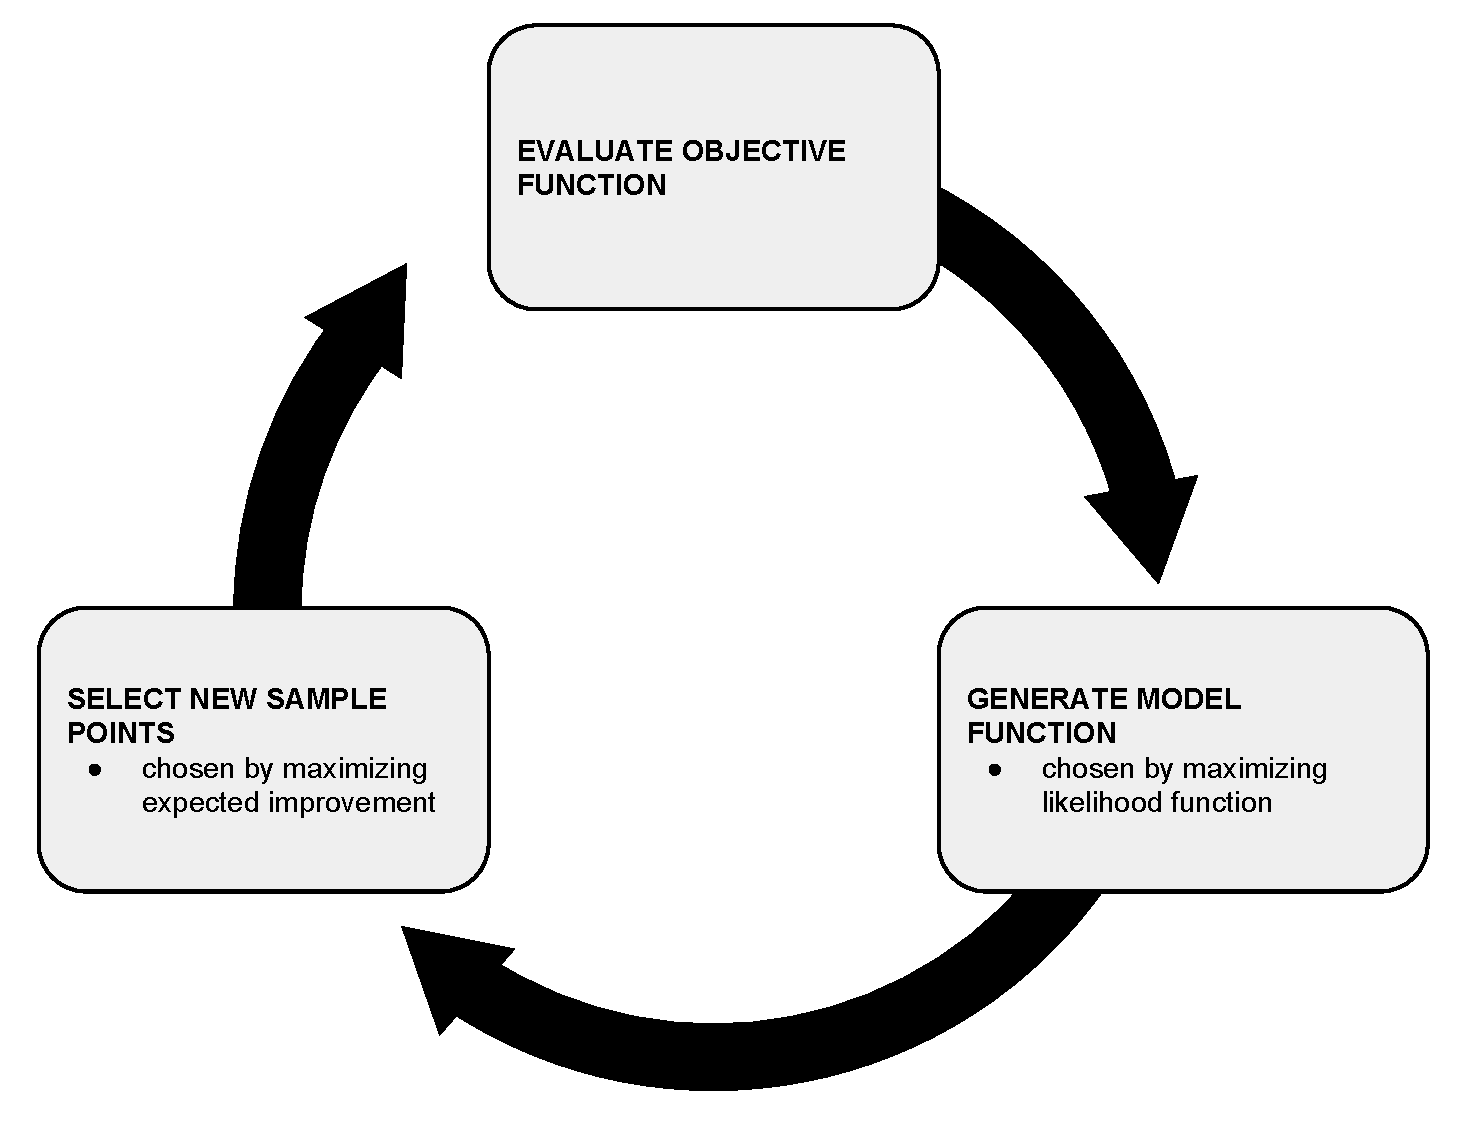
\includegraphics[width=0.8\textwidth]{EGO_cycle_v1}
	\caption{the three stages of the EGO process}
	\label{fig:ego_cycle}

\end{figure}

This steps proceed in a cycle until a global optimum is found.


\section{The Predictor Function}

The predictor function used by the EGO algorithm has also been called the DACE model, for ``design and analysis of computer experiments''. The starting point of the DACE model is parameterized distance function for points in input-space,

\begin{equation} \label{eq:dist}
d(\mathbf{x},\mathbf{x'})=\sum_{h=1}^k \theta_h |x_h-x'_h|^{p_h},
\end{equation}
where $\mathbf{x}$ and $\mathbf{x'}$ are $k$-dimensional vectors. The parameters $\theta_1,...,\theta_k \equiv \mathbf{\theta}$ and $p_1,...,p_k\equiv \mathbf{p}$ effectively define a particular DACE predictor function \footnote{Jones et al p. 460 describes how the two additional parameters, the output $y$'s mean and standard deviation, can be predicted from }. When using the DACE predictor, then, the second stage of the EGO algorithm process diagrammed in Fig. \ref{fig:ego_cycle} consists of choosing $\mathbf{p}$ and $\mathbf{\theta}$ in a manner that best fits whatever data is known about the objective function. Before we can discuss the selection of these parameters, we must understand how they are used to generate a predictor function.

Intuitively, the DACE predictor works by correlating the output of the objective function with variation along each (assumed-to-be-) independent dimension of the input space. This correlation function is defined as simply the negative exponent of the parameterized distance:

\begin{equation} \label{eq:corr}
Corr(\epsilon (\mathbf{x}),\epsilon (\mathbf{x}')) = e^{-d(\mathbf{x},\mathbf{x}')}
\end{equation}

This correlation function behaves as we wish it would. In the original words of Jones et al, ``... when the distance between $\mathbf{x}^i$ and $\mathbf{x}^j$ is small,
the correlation is near one. Similarly, when the distance between the points is large,
the correlation will approach zero.


We define the correlation matrix $\mathbf{R}$ as the $n\times n$ matrix, where
\begin{equation} \label{eq:R}
\mathbf{R}_{(i,j)} = Corr(\epsilon (\mathbf{x}^{(i)}),\epsilon (\mathbf{x}^{(j)}))
\end{equation}




between objective function values at different points in input space\footnote{Precisely, the DACE predictor deals not with correlation between objective function values, but the deviation of objective function values from the mean.[is that correct?]}. When two points are close in input-space, their function value should be close. The details of this relationship will be sensitive to the data and hand. Thus the starting point of the DACE process is constructing a measure of distance between input values from the already-evaluated input-output pairs. 


First, some definitions and variables. I've copied the conventions of Jones et al.

\begin{description}
  \item[Sample Point]: a point in input space where the blackbox function has already been evaluated
  \item[$n$]: the number of sample points
  \item[$k$]: the dimensionality of input space
  \item[$\X^{(i)}$]: the $i$th sample point (a $k$-vector)
  \item[$\X$]: the vector of sample points ($n$ $k$-vectors, an $n\times k$ matrix)
  \item[$y$]: the objective function
  \item[$\Y$]: the vector of evaluated outputs, i.e. $\Y_i=y(\X^{(i)})$
  \item[$p_i \in $[$1,2$]$], \theta_i \geq 0$: two parameters associated with the $i$th input dimension
\end{description}

Tuning the parameters $\theta_1,...,\theta_k$ and $p_1,...,p_k$ to the empirical data $\X$ and $\Y$ is the real computational task in constructing the DACE predictor.

\subsection{Likelihood} \label{sec:likelihood}

%% The "best linear unbiased predictor"
The parameters $p$ and $\theta$ are chosen by maximizing the likelihood function,

\begin{equation} \label{eq:likelihood}
\frac{1}
  {(2\pi\sigma^2)^{n/2}|\mb{R}|^\frac{1}{2}}\ 
exp \left 
  [ -\frac
    {(\mb{y}-\mb{1}\mu)'\mb{R}^{-1}(\mb{y}-\mb{1}\mu)}
    {2\sigma^2} 
\right ]
\end{equation}


Where the best estimates of $\mu$, $\sigma^2$ are,

\begin{equation} \label{eq:mu_hat}
\hat{\mu}=\frac
	{\mb{1}'\mb{R}^{-1}\mb{y}}
	{\mb{1}'\mb{R}^{-1}\mb{1}},
\end{equation}


and,

\begin{equation} \label{eq:sig_hat}
\hat{\sigma}^2=\frac
	{(\mb{y}-\mb{1}\hat{\mu})'\mb{R}^{-1}(\mb{y}-\mb{1}\hat{\mu})}
	{n}.
\end{equation}

Plugging Eqs \ref{eq:mu_hat, eq:sig_hat} into Eq. \ref{eq:likelihood}, gives the concentrated likelihood function that is in optimized to fit the parameters $p$ and $\theta$ to a given dataset.

\subsection{Distance and Correlation Between Sample Points}




\subsection{Predictor}\label{sec:blup}The best linear unbiased predictor of the function's output at $\mb{x^*}$ is,


\begin{equation} \label{eq:blup}
\hat{y}(\mb{x^*})=\hat{\mu} + \mb{r}'\mb{R}^{-1}(\mb{y}-\mb{1}\mu)
\end{equation}



\subsection{Examples}\label{sec:dace_ex}
Any application of the DACE model requires an initial set of sample points. Jones et al use the heuristic of sampling 




\section{Choosing the Next Sample Point}
Here, I'll apply the algorithm to a very simple case where

\bibliographystyle{apalike}
\bibliography{thesis}


\end{document}



